\chapter{Opis aplikacji [TODO]}

\section{Folksonomia}

Folksonomia nazywamy krotkę $F := (U,T,R,Y)$, gdzie:
$U$,$T$,$R$ to zbiory skończone, których elementy składają się odpowiednio z użytkowników, tagów i dokumentów. $Y$ jest relacją “przypisania tagu” pomiędzy tymi elementami $Y < U \times T \times R$

Użytkownicy i tagi identyfikowani są na podstawie ich unikalnych nazw własnych. Dokumenty mogą być różnymi danymi: stronami www, zdjęciami, plikami np: pliki pdf. Ta praca bazuje na danych pobranych z systemu delicous, które w zdecydowanej większości są stronami www. Dane które nie są stroną www nie są brane pod uwagę w tej pracy. 

\section{Architektura}

\subsection{Zbieranie danych:}

Dane pobierane są na kilka sposobów. Głównym źródłem nowych danych jest kanał RSS strony delicous. Dodatkowo dla użytkowników i dokumentów które są już zapisane w bazie danych, co powien przedział czasu, sprawdzane jest czy nie zostały dla nich dodane nowe wpisy na stronie delicous.

\subsection*{Nowe dane}

Serwis delicous daje użytkownikom 
Kanał RSS delicous zawiera dane ostatnio dodane przez użytkowników serwisu delicous. 


Każdy wpis zawiera informacje o użytkowniku, który ostatnio dodał daną strone, tagi, adres strony i adres kanału rss tej strony. Każdy z kanałów RSS


\begin{enumerate}
\item Crawler Delicous:

\begin{itemize}
\item sprawedza najnowsze dane dodawane przez wsyzstkich uzytwkoników na głównej stronie delicous.
\item sprwadza popularne strony dodawane przez uzytwkoników. To czy dana strona znajdywała sie wśród popularnych jest równiez zapusywanie w bazie danych.
\item update: sprwadzanie danych ze strony uzywtkoników którzy już są dodani jak również sprawdzanie czy strony ktore juz były dodane nie otrzymały nowych tagów i czy nie było innych uzytkowników którzy dana strone dodali równiez (pozwala to na szybkie zwiekszenie danych, ale rowniez moze spowodowac potencjalne problemy: moze to spowodowac ze dane ktore beda w bazie bedą do siebie podobne - ci sami uzytwkonicy dodaja podobne strony, w podobnej tematyce, z drugiej strony,  osoby ktorzy dodali dana strone, mogą mieć podobne preferencje)
\end{itemize}

Najnowsze dane pochodzą z przeglądania głownego RSS’a strony. Po sparsowaniu danych, wyciagane sa nowe strony. Kazdy z tych nowych URL’i posiada swoja strone na delicous, na ktorej przechowywane sa dane o uzytkownikach ktorzy dodali i tagach uzytych. Przegladane zostaje



\item Crawlery innych serwisów społecznościowych:

w swoim systemie korzystam z serwisów tweeter, facebook, digg. Dostarczaja one API ktore pozwala sprwadzic ile uzytkwoników udosteponiło dana strone. Działaja one niezaleznie od siebie. Sprawdzane są jednoczesnie nowo dodane do systemu strony jak również przeprowadzany jest update pozostałych

\item Lucene:




\item cache:

\begin{itemize} 
\item statystyki -- co powiem okreslony czas na bazie danych robiony jest update statystyk. Wyliczanie statystyki powoduja jednak duze obciazenie bazy danych. Najwiekszym problemem nie jest obciazenie ale
obencie wyliczane statystyki:
\begin{itemize} 
    \item  dla uzytkownika:
	\begin{itemize} 
          		\item  ilosc dodanych dokumentow
	          	\item ilość uzywanych tagów,
	          	\item najczesciej uzywane tagi
	\end{itemize}
    \item  dla dokumentu:
	\begin{itemize} 
	          	\item ile razy dodany przez uzytkowników
	          	\item ile razy został otagowany
	          	\item ile razy został otagowany rozymi słowami
	          	\item najczęstrze tagi uzywane do opisania tego dokuemtnu
	\end{itemize}
    \item  dla tagów
	\begin{itemize} 
	          \item  ile razy uzywany przez roznych uzytwkoników
	          \item  ile razy uzywany w ogóle.
	          \item  na ilu roznych dokumentach zostal uzyty
	          \item  najczestrze dokuemtny opisane tym tagiem
	          \item  uzytkownicy, uzywajacy najczesciej jego
	\end{itemize}
\end{itemize}


\end{itemize}

\item cache wyszukiwarki: w tabeli documents dodawane są rowniez dodatkowe informacje ktore są wypisywane w momencie kiedy wyszukiwarka zwroci wynik, a ich wyliczanie w czasie podawania wyniku dla uzytkownika bylo by zbyt czasochłonne. Tymi dodatkowymi rzeczami są: często używane tagi, ilość użytkowników który dany tag dodała. Dane te są od razu sformatowane i gotowe do wypisane w przeglądarce

\end{enumerate}

\section{Baza danych}

Jako serwer bazy używany jest MySQL 5.1. Komunikacja między aplikację a bazę danych odbywa się za pomocą frameworku Hibernate. Framework ten zapewnia translację danych z relacyjnej bazy danych na obiekty używane w aplikacji. 


\begin{figure}[h]
\centering
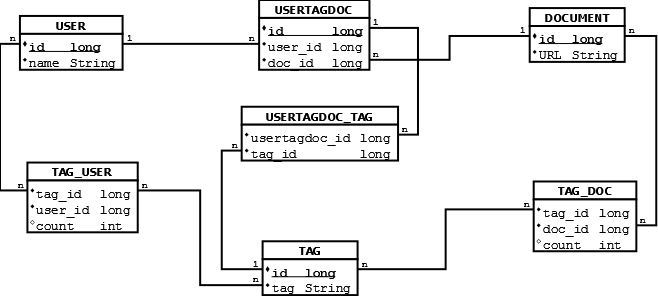
\includegraphics[width=1\textwidth]{db.png}
\caption{Baza danych}
\label{fig:db_fig}
\end{figure}


\subsection*{Opis tabel:}
\begin{itemize}
	\item USER: tabela zawiera dane użytkowników, ich $id$ i unikalną nazwę pobraną z serwisu delicous.
	\item DOCUMENT: tabela zawiera dane o dokumentach. $URL$ który reprezentuje dokument jest unikalny. Ponieważ adresy stron po pominięciu ostatniego slasha/backslasha prowadzą do tych samych witryn, przy sprawdzaniu unikalności linku brane pod uwagę są wszystkie kombinacje adresów.
	\item TAG: tabela zawierająca adnotacje stron.
	\item USERTAGDOC i USERTAGDOC\_TAG: są to tabele które służą do zapisania w bazie danych relacji nadania $k$ tagów: $t_n, t_{n+1}, \dots, t_{n+k}$ przez użytkownika $user_j$  dokumentowi $doc_m$. Dodatkowo wartość $k$: ilość przypisanych tagów, zapisana jest w polu $count$.
	\item TAG\_USER i TAG\_DOC: tabele zawierające redundantne dane. TAG\_USER zwiera informacje o ilości dokumentów opisanym tagiem $tag_k$ przez użytkownika $user_n$. Druga tabela zawiera informacje o liczbie przypisań tagu $tag_k$ do dokumentu $doc_m$. Tabele te są wykorzystywane dla szybszego zbierania danych dla algorytmów Adapter PageRank i SocialPageRank.
\end{itemize}


\subsection*{Tagi:}
Tagi nie są dodawane do bazy danych w postaci dokladnie uzyskanej ze strony delicous. Wiele z nich wymaga paru przekształcen. Podstawowym jest usuniecie białych znaków z początku i konca słowa. Dodawkowo, wiekszość tagów, zaczyna lub kończy się na znakach specjalnych, lub znajduje sie w cudzysłowiu czy też kończy się znakiem przecinka. Dla przykładu:

\begin{itemize} 
    \item @java
    \item  @@java
    \item  \#java
    \item  java@
    \item  “tag” / “tag / tag”
    \item  tekst, / ,tekst
\end{itemize}


\section{Interface użytkownika}
interface uzytwkonika napisany jest przy pomocy technologi google-web-toolkit.
głowny panel zawiera u góry zakładki, które pozwalaja na przemieszczenie sie miedzy wyszukiwarką, statystykami, tagami, innymi informacjami.

uzytkownik po wczytaniu zapytaniu i nacisnieciu ENTER otrzymuje wyniki zapytania.

\section{Lucene}

Lucene jest biblioteką napisaną w Javie. Biblioteka ta jest w stanie indeksować dużą ilość dokumentów z różnych źródeł i przeprowadzać wyszukiwania w tych tekstach. W tym systemie, framework Lucene przechowuje źródła stron, o których informacje zostały pobrane z serwisu delicous i zapisane w bazie danych. 



\subsection{Pobieranie stron}

W pewnych odstępach czasu, wątek odpowiedzialny za indeksowanie stron sprawdza czy w bazie danych tabela dokuemtn nie ma informacji o nowych wpisach. Z bazy danych pobrane są informacje o adresach tych stron. Następnie dla każdego adresu URL zostaje pobrana treść strony na którą wskazuje. Strona WWW następnie zostaje oczyszczona ze znaczników HTML, i przekazane do frameworku lucene do zaindeksowania. Jeśli wszystkie czynności zakończą się powodzeniem, w bazie danych zostaje odnotowana informacja o posiadaniu na dysku danego dokumentu. Rysunek \ref{fig:lucene_index_fig} przedstawiony jest cały proces pobierania i przetwarzania danej strony.

\begin{figure}[htb]

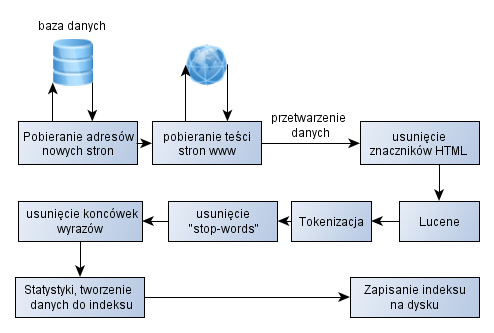
\includegraphics[width=1\textwidth]{lucene_indeksing.png}
\caption{Lucene: pobieranie danych i indeksowanie}
\label{fig:lucene_index_fig}
\end{figure}

Do Lucene zapisywane są następujące informacje: identyfikator $id$ dokumentu z bazy danych, oraz przetworzony tekst strony WWW. Przechowywanie identyfikatora dokumentu w danych Lucene pozwala późniejsze powiązanie wyników wyszukiwania z odpowiednim rekordem w bazie danych. 

W czasie indeksowania biblioteka Lucene wykonuje wiele czynności które pozwalają jej później szybko wyszukiwać informację. Główne z nich to:
\begin{itemize}
\item Tokenizacja: tekst zostanje przetworzony na ciąg tokenów,
\item usunięcie końcówek wyrazów,
\item usunięcie 'stop-words' z tekstu, czyli słów nie mających dużego znaczenia przy wynikach wyszukiwania,
\item statystyki, np: wystąpienia słów w dokumencie, odległości od siebie
\end{itemize}

\subsection{Wyszukiwanie}

Czas wyszukiwania zapytania w dokumentach przechowywanych Lucene jest szybkie. Przy małej, poniżej 1GB danych, wyszukiwanie następuje praktycznie w czasie rzeczywistym. Zapytanie jest przekazywane do frameworku, w którym jest one przekształcane na tokeny. Dla zapytania $q$ i dla każdego dokumentu $d$ wyliczana jest wartość funkcji $score(q,d)$. Wynikiem są dokumenty posortowane wg. wyniku tej funkcji.

$score(q,d) =   coord(q,d)  *  queryNorm(q) * \sum_{t \text{ in } q}  \bigg( tf(t\text{ in } d)  *  idf(t)^2  *  getBoost(t) *  norm(t,d) )$

gdzie:
\begin{itemize}
	\item coord(q,d): funkcja zwraca wartości zależne od miejsca występowania i odległości od siebie tokenów zapytania w dokumencie.
	\item queryNorm(q): funkcja normalizująca wyniki zapytania
	\item tf(t in d): funkcja wyliczająca częstość występowania danego termu w dokumencie
	\item idf(t) : funkcja wyliczająca częstość występowania termu we wszystkich dokumentach.
	\item getBoost(t) - Lucene pozwala na zwiększenie wagi niektórych termów. Nieużywane w tej aplikacji.
\end{itemize}

Lucene ocenia dokumenty głównie na podstawie funkcji TF-IDF. Każdy dokument reprezentowany jest przez wektor, składający się z wag słów występujących w tym dokumencie. TFIDF informuje o częstości wystąpienia termów uwzględniając jednocześnie odpowiednie wyważenie znaczenia lokalnego termu i jego znaczenia w kontekście pełnej kolekcji dokumentów.


